In this section we will go over the results of the various experiments we have concocted. The results will be evaluated in two separate ways. For each experiment there are two models, the "final" model that was saved after all training was finished, and the "minloss" model which was saved during training when the model achieved the lowest loss. With the last experiment being the exception, all results shown are from the "final" models.\\

\noindent
The first evaluation will be on a structural classification dataset, which will be a qualitative analysis in which we perform t-distributed stochastic neighbor embedding (TSNE) dimensionality reduction on the data, and see whether it is able to cleanly separate the different types of protein structures. TSNE is preferred here over something like principal component analysis (PCA) due to this non-linearity of the reduction. This evaluation will be performed on the structural classification dataset. While using a classification method like k-nearest neighbors (KNN) might seem intuitive to quantitatively evaluate this, the non-linearity means that neither distance nor density is preserved between data points. We will also look at the next token prediction accuracy for the LSTM, but because we want to quantify how well it represents the proteins, this is not necessarily a good way to do that. It will mostly be used for comparison to see if there are any interesting insights.\\

\noindent
The second evaluation will be on the stability dataset. This evaluation will be quantitative, using Spearman's rank correlation coefficent. This coefficient measures the degree to which the relationship between two inputs can be described using a monotonic function. This means that having a high spearman correlation is equivalent to having a highly descriptive representation. It does not necessarily mean that the linear regression model we have trained provides good results in and of itself, since the coefficient does not describe a 1:1 correlation. This can be seen in figure ~\ref{fig:spearman}.

\begin{figure}[!ht]
  \centering
  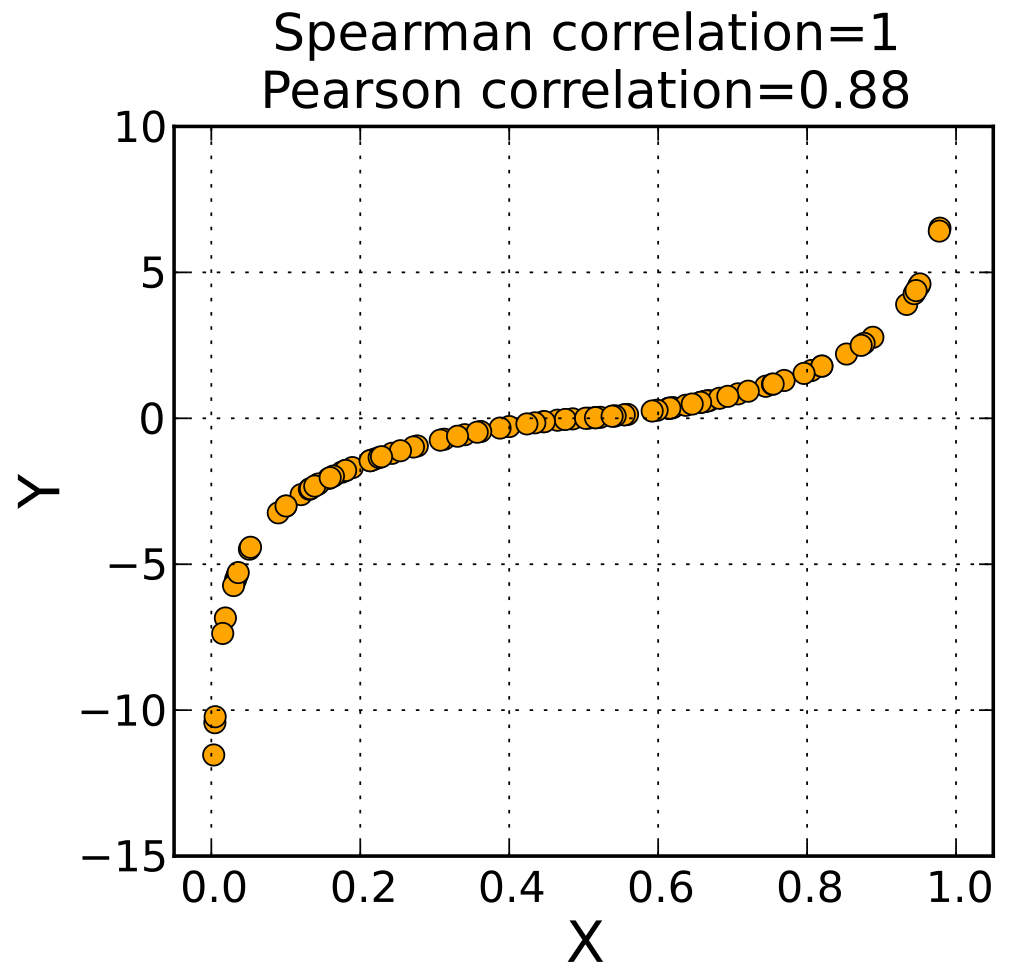
\includegraphics[width=0.4\linewidth]{latex/imgs/spearman_fig.png}
  \caption{Graph showing that high spearman correlation does not necessarily mean a good score. Image source:\cite{spearman}}\label{fig:spearman}
\end{figure}

\subsection{LSTM experiments}

\subsubsection{Layers vs no layers}
\begin{figure}[h]
	% Accuracy on test set: 12.43%, loss 2.84
  	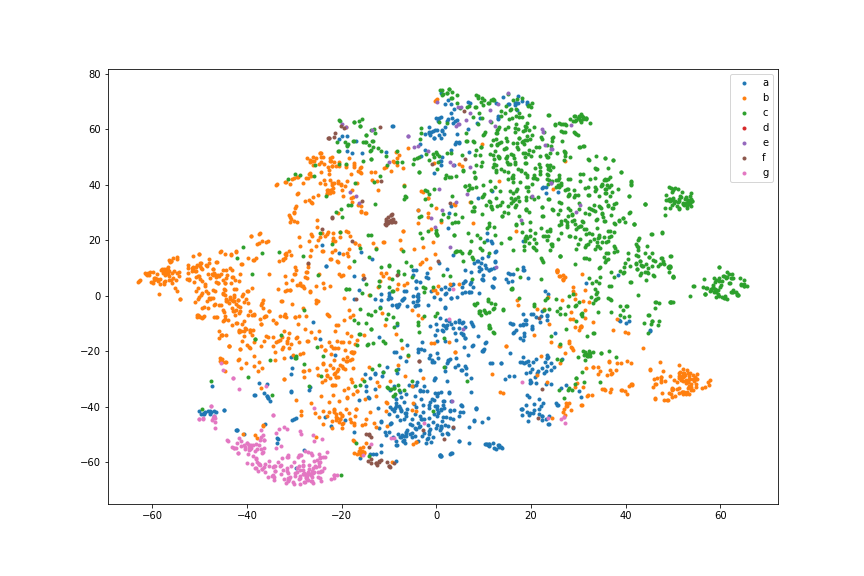
\includegraphics[width=0.4\linewidth]{latex/imgs/tsne_1_layer_with_schedule_512_final.png}
  	% Accuracy on test set: 13.03%, loss 2.83
  	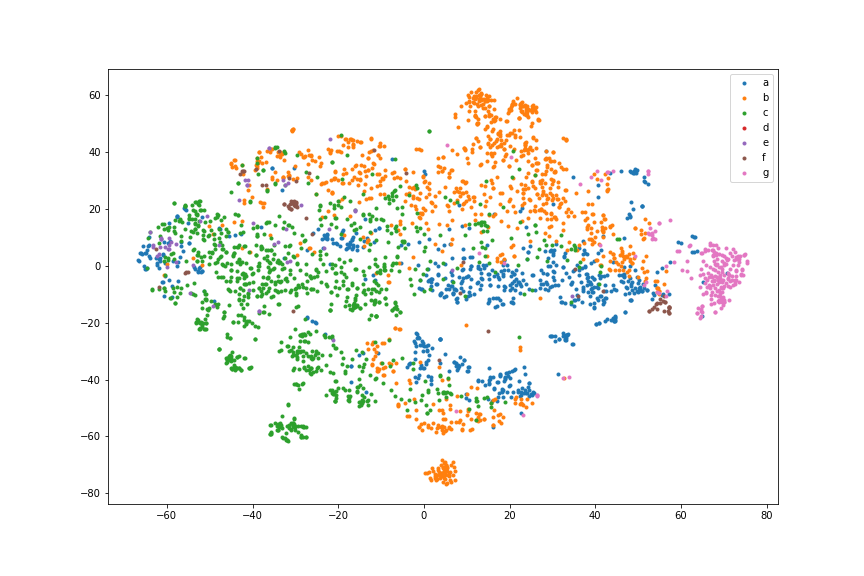
\includegraphics[width=0.4\linewidth]{latex/imgs/tsne_2_layer_no_drop_final.png}
	\caption{TSNE dimensionality reduction of the two models. Left is 1-layer, right is 2-layer}
\end{figure}

\begin{figure}[h]
	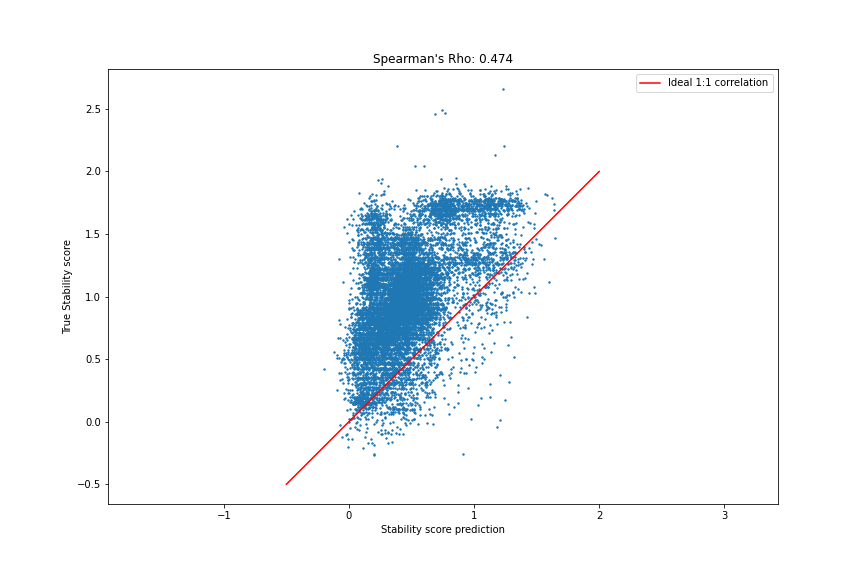
\includegraphics[width=0.4\linewidth]{latex/imgs/spearman_1_layer_with_schedule_512_final.png}
	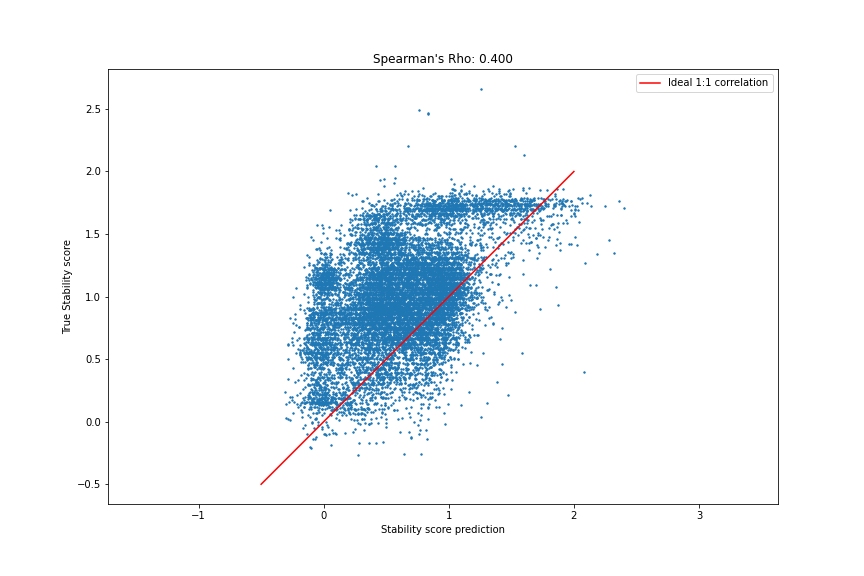
\includegraphics[width=0.4\linewidth]{latex/imgs/spearman_2_layer_no_drop_final.png}
	\caption{Plots used to calculate the Spearman correlation. Left is 1-layer, right is 2-layer}
\end{figure}

\begin{table}[]
\begin{tabular}{|l|l|l|l|}
\hline
        & Next token prediction accuracy & Test Loss & Spearman's rho\\ \hline
1-layer & 12.43\%                        & 2.84      & 0.400         \\ \hline
2-layer & 13.03\%                        & 2.83      & 0.428         \\ \hline
\end{tabular}
\end{table}

% TSNE plots
\begin{figure}[!ht]
  \centering
  % Accuracy on test set: 13.02%, loss 2.82
  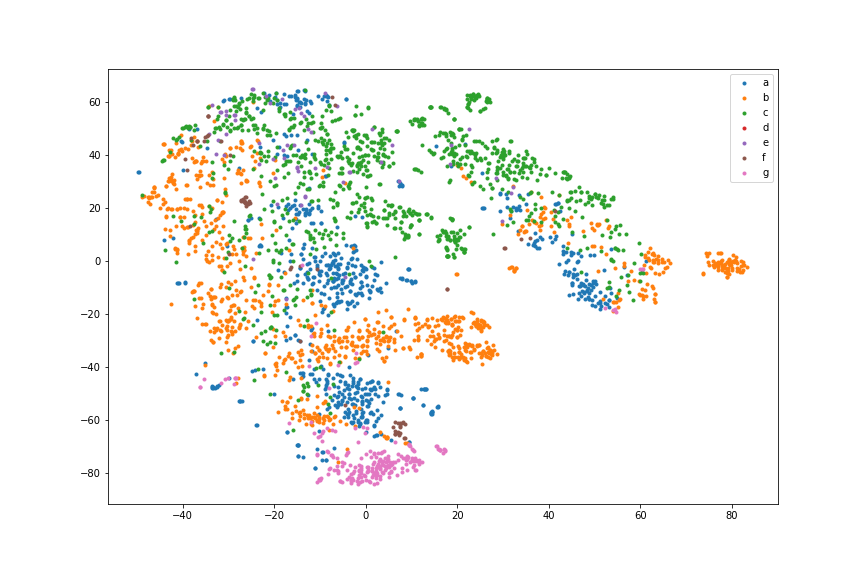
\includegraphics[width=0.4\linewidth]{latex/imgs/tsne_2_layer_05_drop_final.png}
  % Accuracy on test set: 13.03%, loss 2.82
  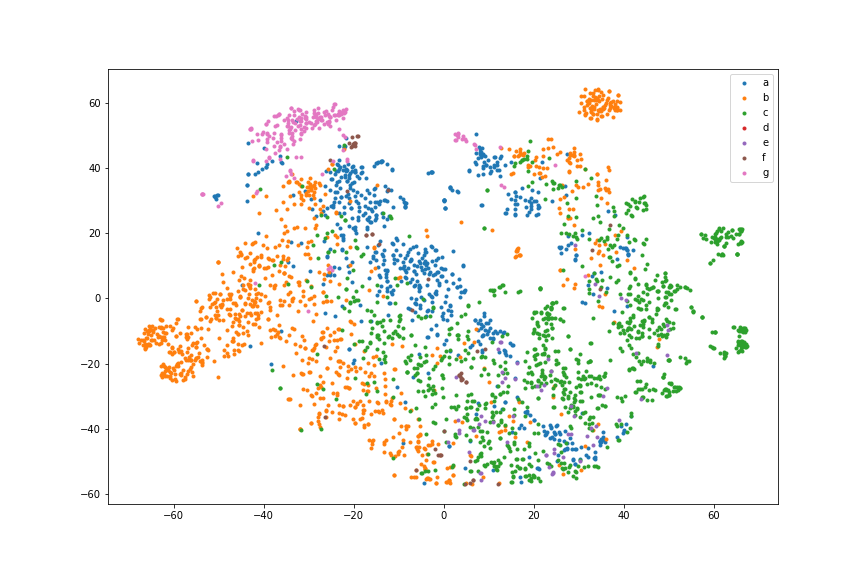
\includegraphics[width=0.4\linewidth]{latex/imgs/tsne_2_layer_05_drop_minloss.png}
  \caption{TSNE dimensionality reduction. Left is final model, right is minloss model.}
\end{figure}
\begin{figure}[!ht]
  \centering
  % 0.518 and 0.539
  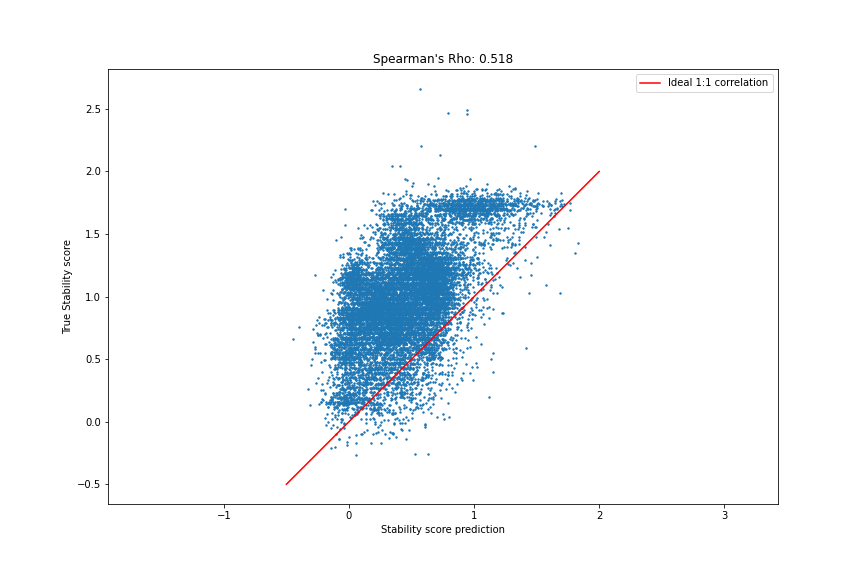
\includegraphics[width=0.4\linewidth]{latex/imgs/spearman_2_layer_05_drop_final.png}
  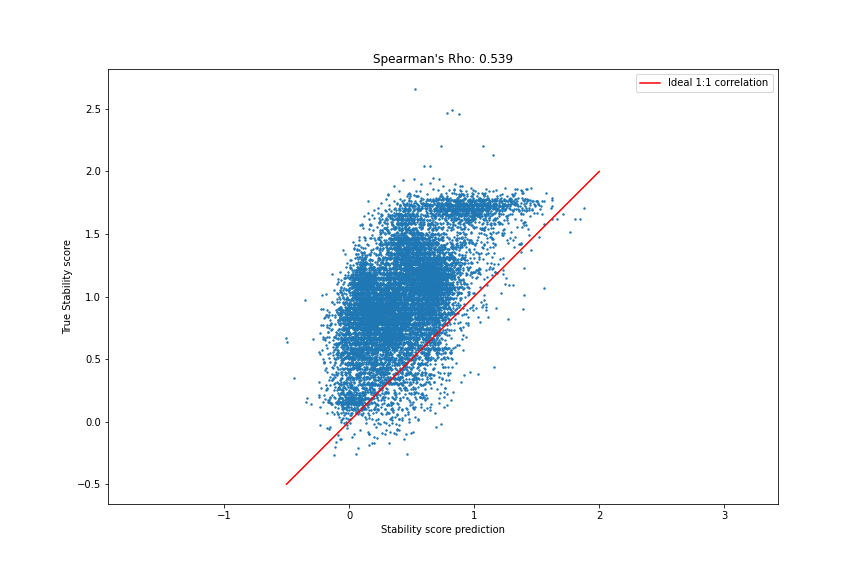
\includegraphics[width=0.4\linewidth]{latex/imgs/spearman_2_layer_05_drop_minloss.png}
  \caption{Plot showing the values the spearman correlation was calculated from.}
\end{figure}


\begin{figure}[!ht]
  \centering
  % Accuracy on test set: 13.03%, loss 2.83
  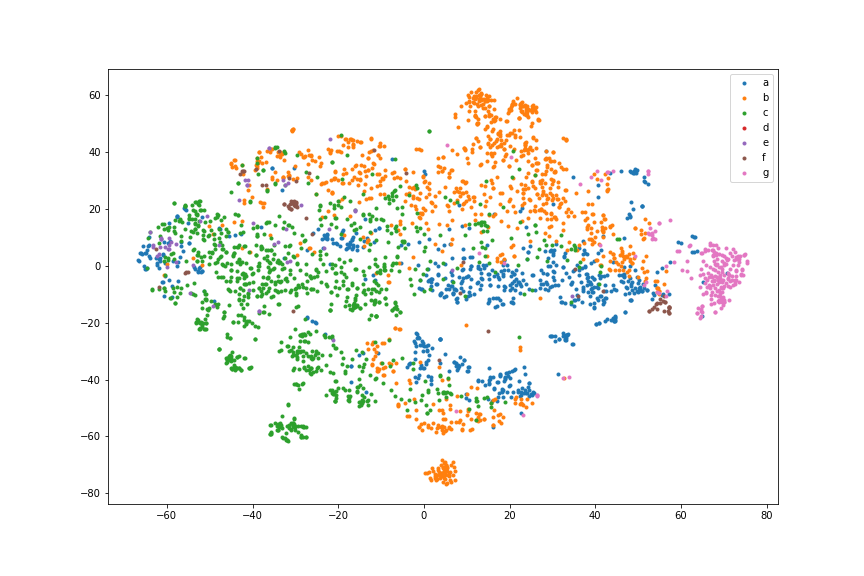
\includegraphics[width=0.4\linewidth]{latex/imgs/tsne_2_layer_no_drop_final.png}
  % Accuracy on test set: 13.78%, loss 2.81
  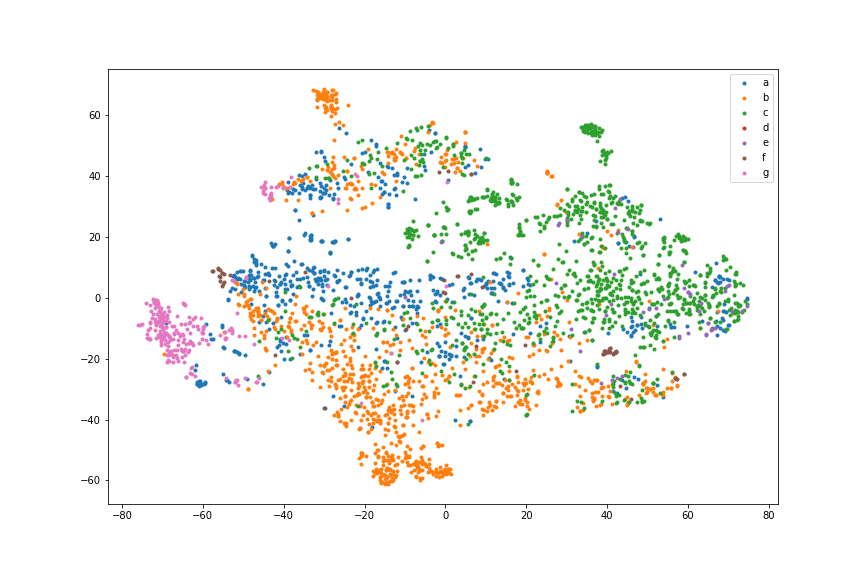
\includegraphics[width=0.4\linewidth]{latex/imgs/tsne_2_layer_no_drop_minloss.png}
  \caption{Graph showing that high spearman correlation does not necessarily mean a good score. Image source:\cite{spearman}}
\end{figure}
\begin{figure}[!ht]
  \centering
  % Accuracy on test set: 13.34%, loss 2.83
  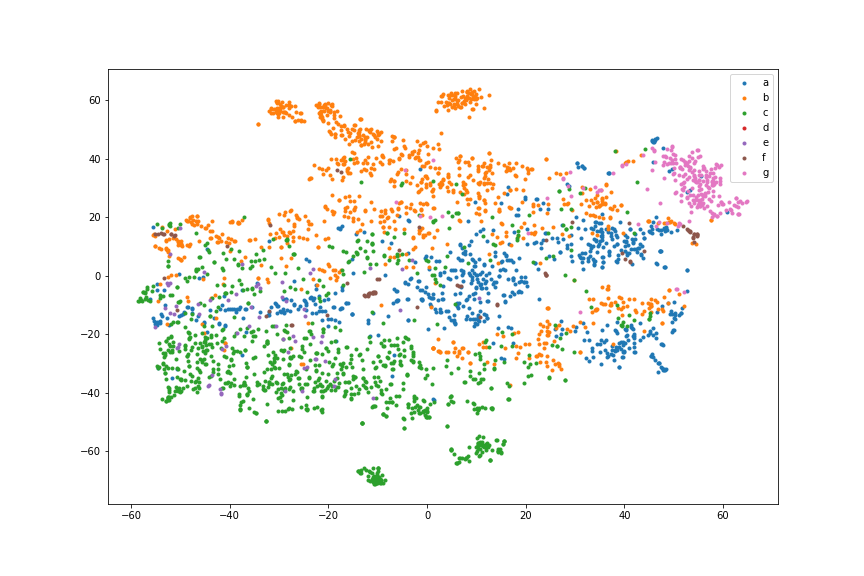
\includegraphics[width=0.4\linewidth]{latex/imgs/tsne_1_layer_no_schedule_512_final.png}
  % Accuracy on test set: 13.36%, loss 2.83
  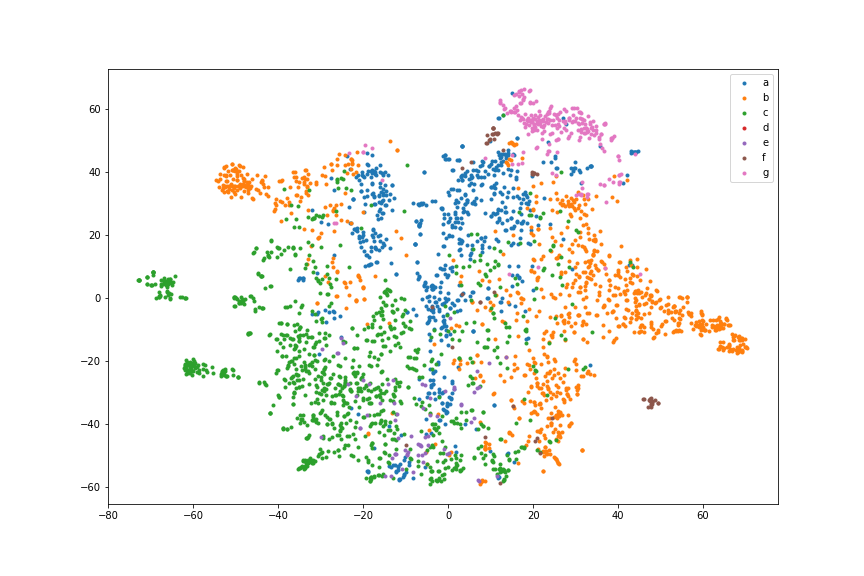
\includegraphics[width=0.4\linewidth]{latex/imgs/tsne_1_layer_no_schedule_512_minloss.png}
  \caption{Graph showing that high spearman correlation does not necessarily mean a good score. Image source:\cite{spearman}}
\end{figure}
\begin{figure}[!ht]
  \centering
  % Accuracy on test set: 12.43%, loss 2.84
  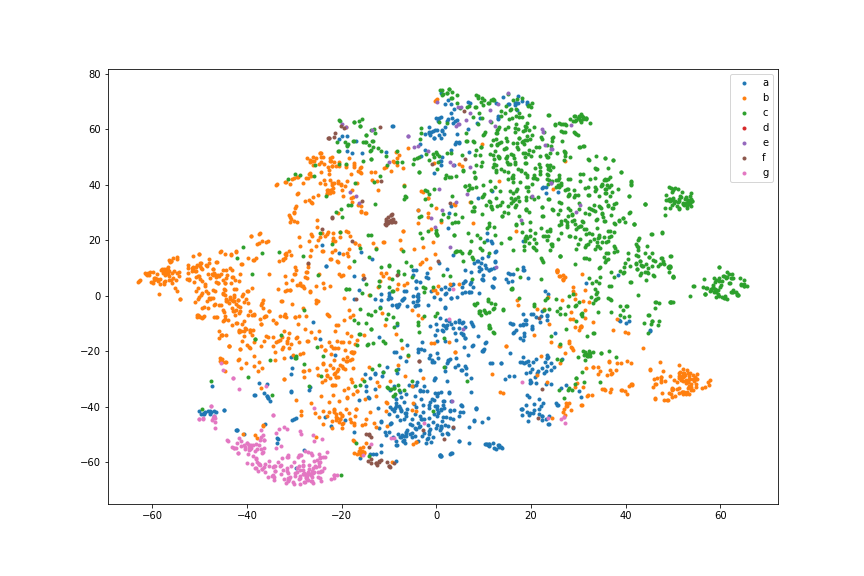
\includegraphics[width=0.4\linewidth]{latex/imgs/tsne_1_layer_with_schedule_512_final.png}
  % Accuracy on test set: 12.43%, loss 2.85
  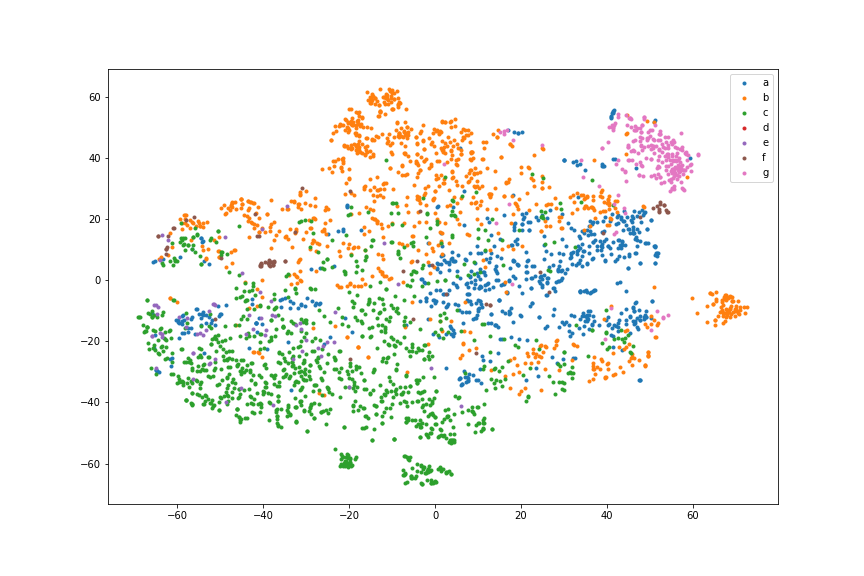
\includegraphics[width=0.4\linewidth]{latex/imgs/tsne_1_layer_with_schedule_512_minloss.png}
  \caption{Graph showing that high spearman correlation does not necessarily mean a good score. Image source:\cite{spearman}}
\end{figure}
\begin{figure}[!ht]
  \centering
  % Accuracy on test set: 11.41%, loss 2.86
  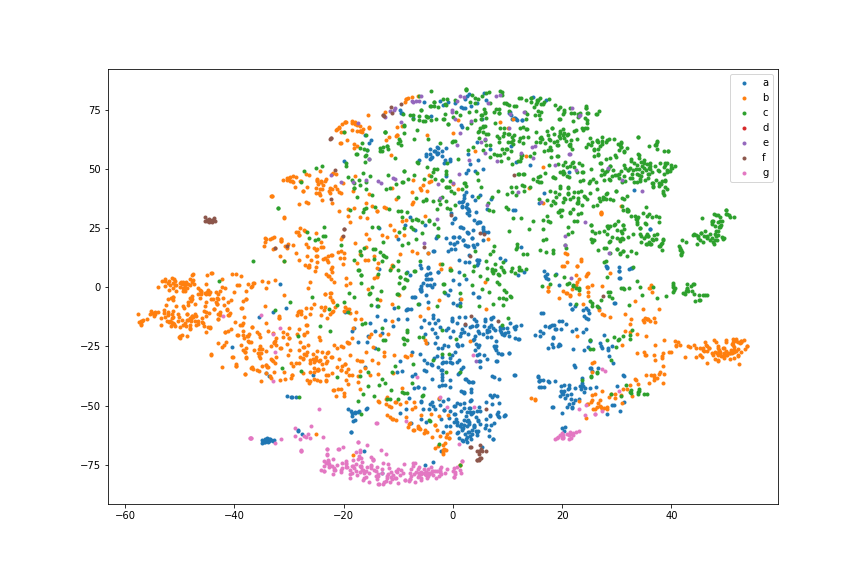
\includegraphics[width=0.4\linewidth]{latex/imgs/tsne_1_layer_with_schedule_256_final.png}
  % Accuracy on test set:  11.40%, loss 2.87
  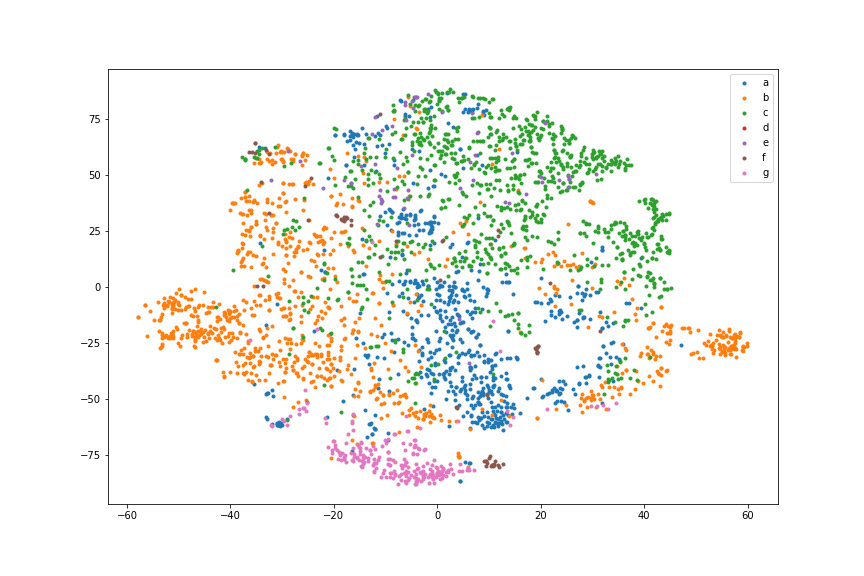
\includegraphics[width=0.4\linewidth]{latex/imgs/tsne_1_layer_with_schedule_256_minloss.png}
  \caption{Graph showing that high spearman correlation does not necessarily mean a good score. Image source:\cite{spearman}}
\end{figure}
\begin{figure}[!ht]
  \centering
  % Accuracy on test set: 14.37%, loss 2.79
  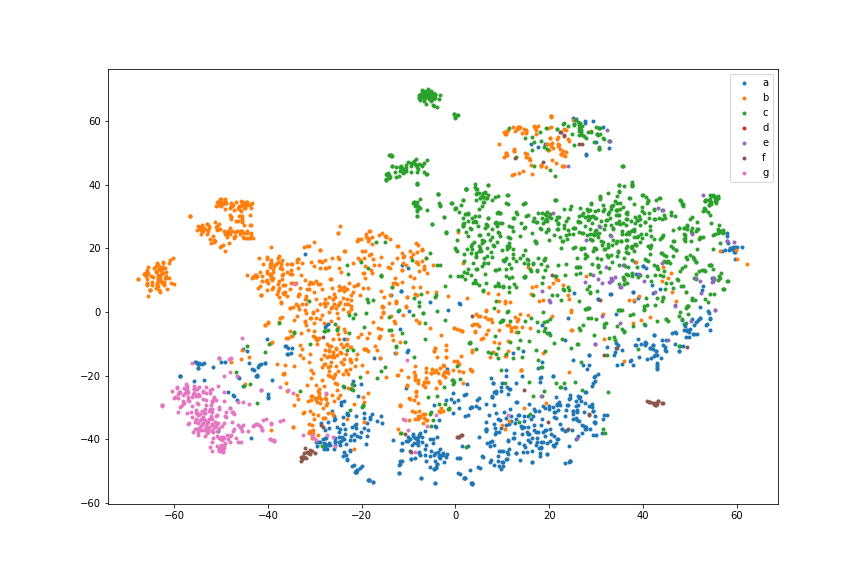
\includegraphics[width=0.4\linewidth]{latex/imgs/tsne_1_layer_with_schedule_1024_final.png}
  % Accuracy on test set:  14.22%, loss 2.80
  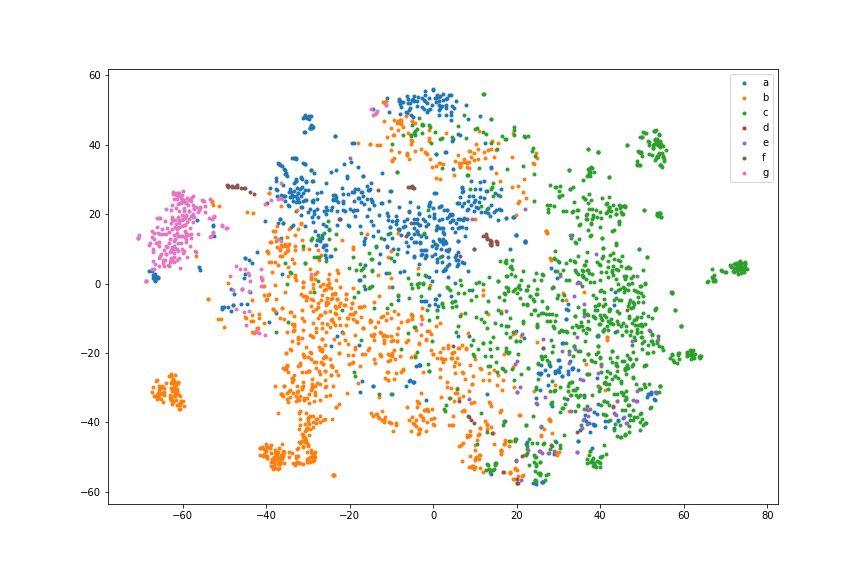
\includegraphics[width=0.4\linewidth]{latex/imgs/tsne_1_layer_with_schedule_1024_minloss.png}
  \caption{Graph showing that high spearman correlation does not necessarily mean a good score. Image source:\cite{spearman}}
\end{figure}

% KIG PÅ SPEARMAN DATA
% Spearman Plots

\begin{figure}[!ht]
  \centering
  % 0.400 and 0.427
  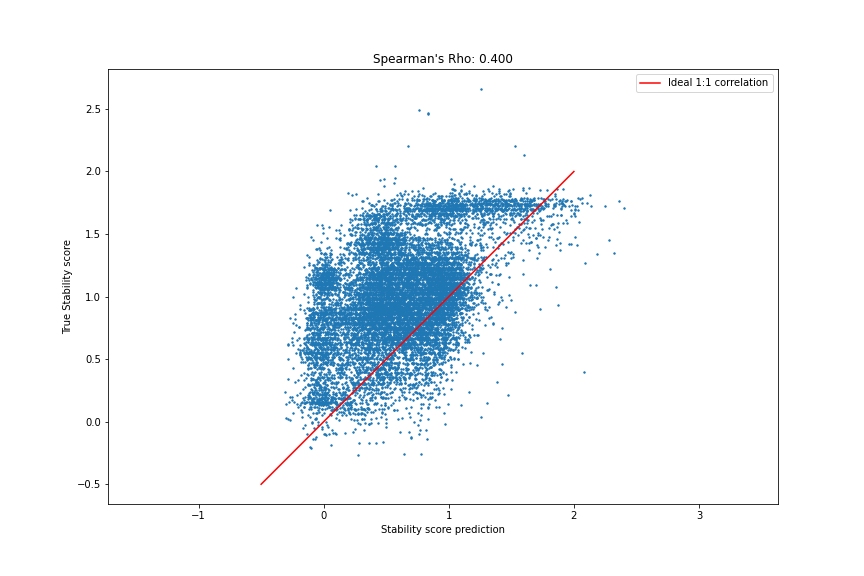
\includegraphics[width=0.4\linewidth]{latex/imgs/spearman_2_layer_no_drop_final.png}
  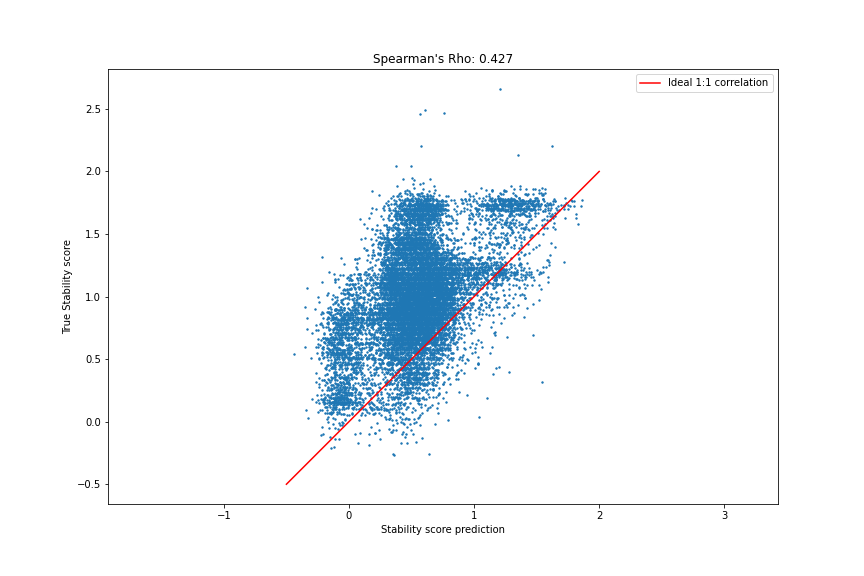
\includegraphics[width=0.4\linewidth]{latex/imgs/spearman_2_layer_no_drop_minloss.png}
  \caption{Graph showing that high spearman correlation does not necessarily mean a good score. Image source:\cite{spearman}}
\end{figure}
\begin{figure}[!ht]
  \centering
  % 0.605 and 0.592
  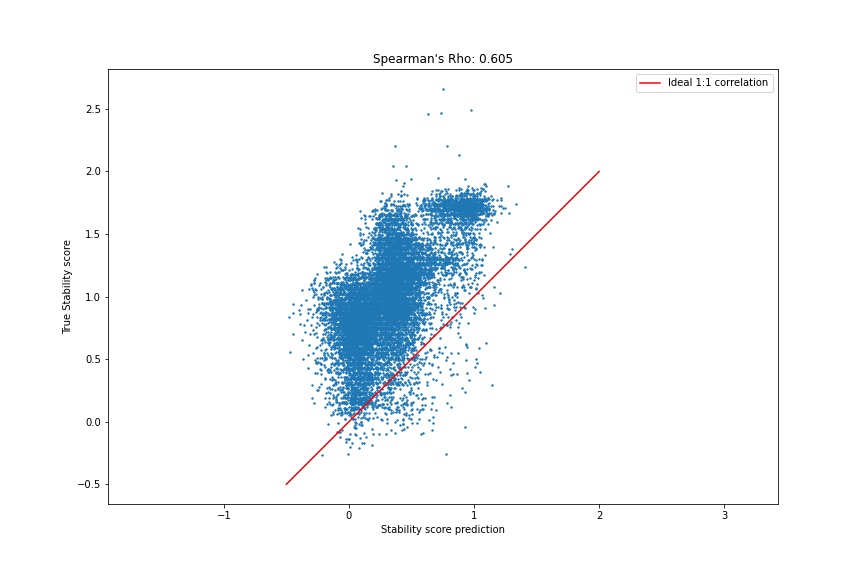
\includegraphics[width=0.4\linewidth]{latex/imgs/spearman_1_layer_no_schedule_512_final.png}
  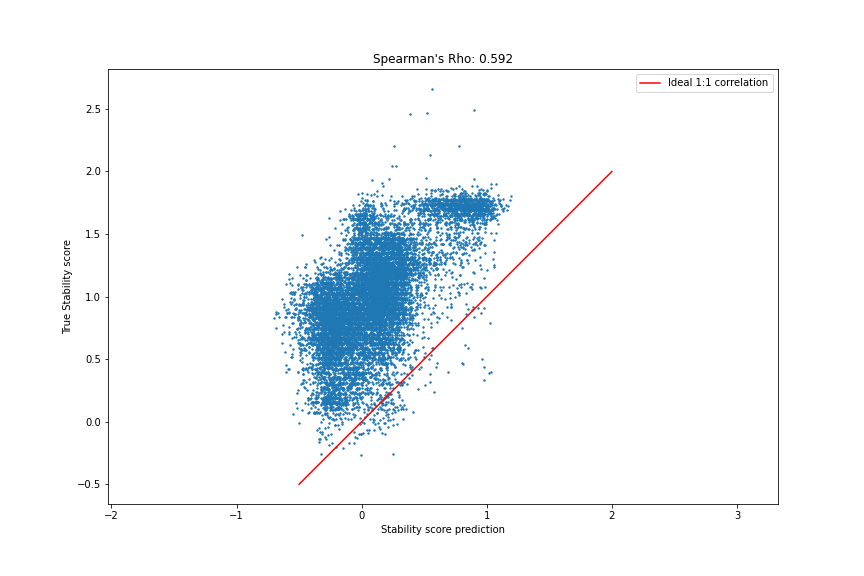
\includegraphics[width=0.4\linewidth]{latex/imgs/spearman_1_layer_no_schedule_512_minloss.png}
  \caption{Graph showing that high spearman correlation does not necessarily mean a good score. Image source:\cite{spearman}}
\end{figure}
\begin{figure}[!ht]
  \centering
  % 0.428 and 0.414
  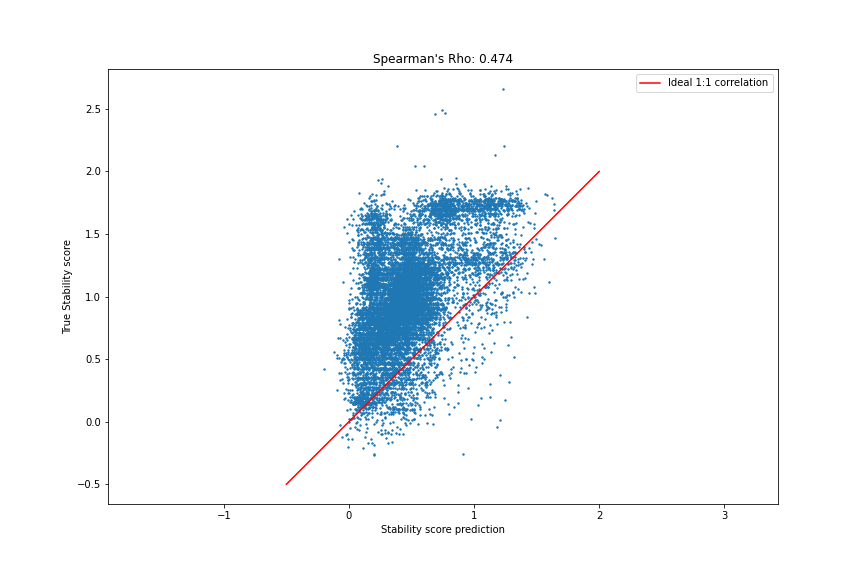
\includegraphics[width=0.4\linewidth]{latex/imgs/spearman_1_layer_with_schedule_512_final.png}
  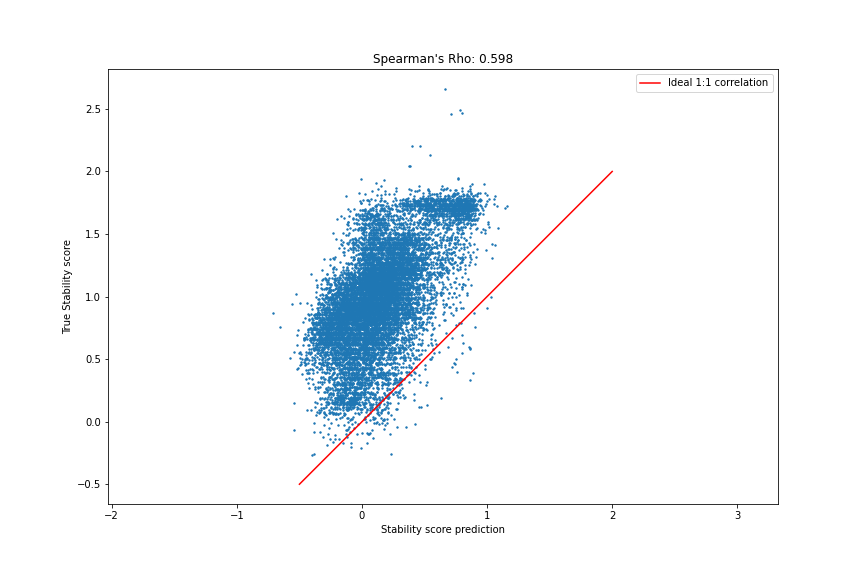
\includegraphics[width=0.4\linewidth]{latex/imgs/spearman_1_layer_with_schedule_512_minloss.png}
  \caption{Graph showing that high spearman correlation does not necessarily mean a good score. Image source:\cite{spearman}}
\end{figure}
\begin{figure}[!ht]
  \centering
  % 0.435 and 0.424
  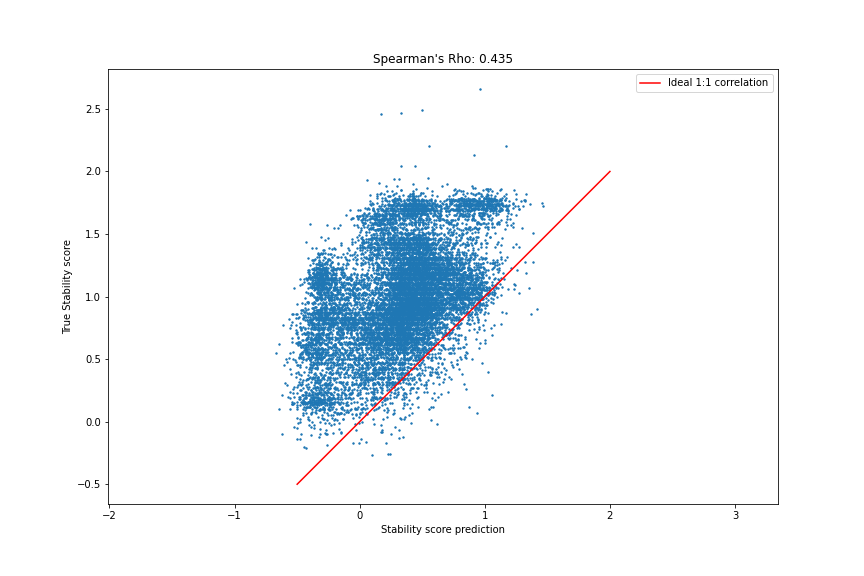
\includegraphics[width=0.4\linewidth]{latex/imgs/spearman_1_layer_with_schedule_256_final.png}
  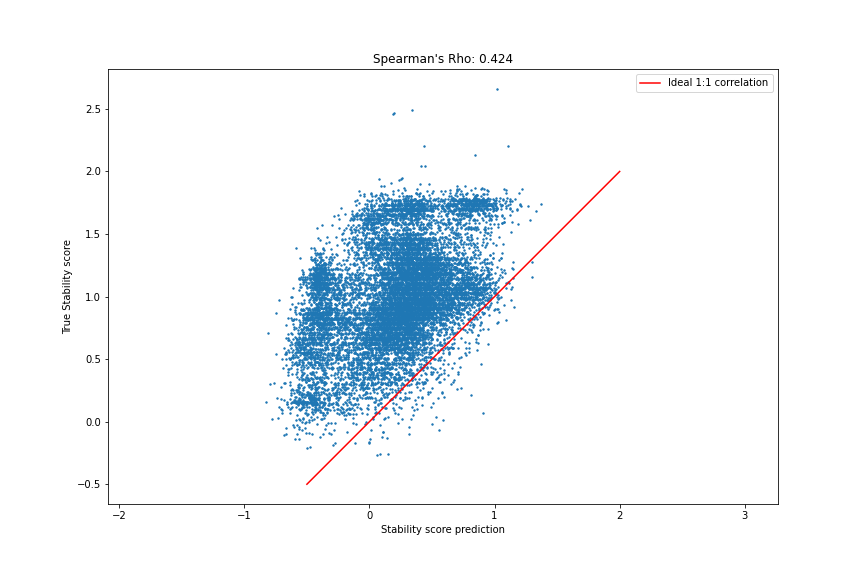
\includegraphics[width=0.4\linewidth]{latex/imgs/spearman_1_layer_with_schedule_256_minloss.png}
  \caption{Graph showing that high spearman correlation does not necessarily mean a good score. Image source:\cite{spearman}}
\end{figure}
\begin{figure}[!ht]
  \centering
  % 0.507 and 0.627
  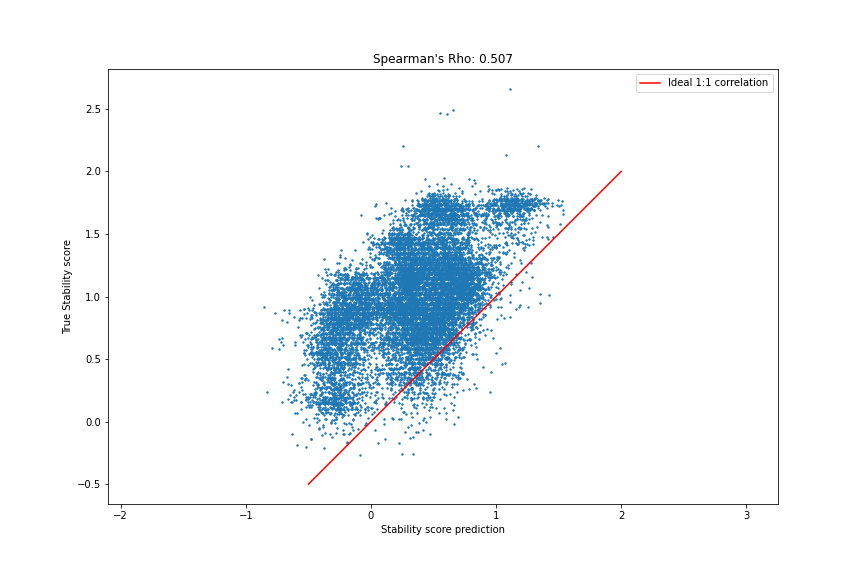
\includegraphics[width=0.4\linewidth]{latex/imgs/spearman_1_layer_with_schedule_1024_final.png}
  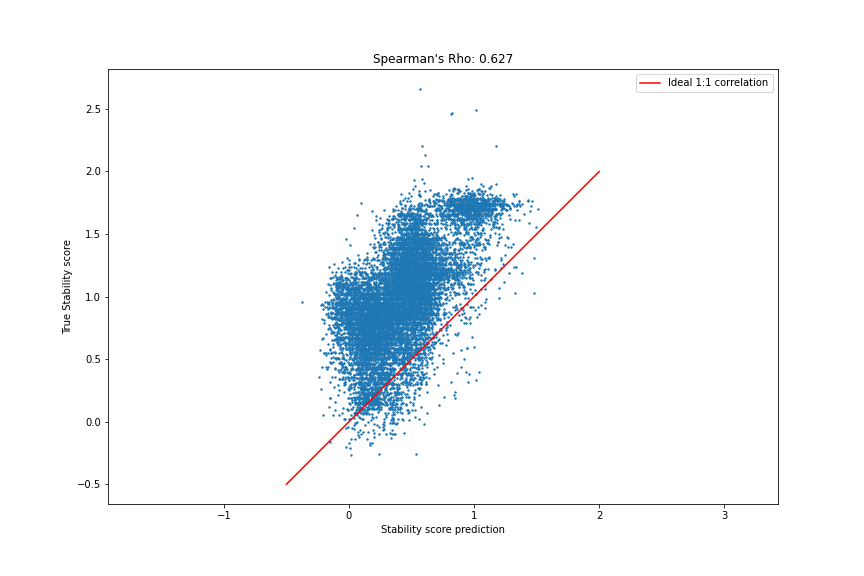
\includegraphics[width=0.4\linewidth]{latex/imgs/spearman_1_layer_with_schedule_1024_minloss.png}
  \caption{Graph showing that high spearman correlation does not necessarily mean a good score. Image source:\cite{spearman}}
\end{figure}

\subsubsection{CNN}
